\begin{SCfigure}%[t]
  \centering
  \caption[Euclidean vs. Curvilinear Distance]{Two ways to measure
    distance: Euclidean vs. Curvilinear. The Euclidean distance from A
    to B is direct ($length=18$). Curvilinear distance from A to B
    follows the path indicated ($length=86$). Each measurement
    approach has a related midpoint, indicated as smaller dots.}
  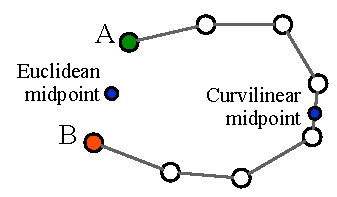
\includegraphics[width=3in]{img/distance-measures.pdf}
  \label{fig:distance-measures}
\end{SCfigure}
